\chapter{系统测试}
\thispagestyle{fancy}
本章介绍系统的测试结果。

\section{测试设置}
系统的测试设置如下:
\begin{itemize}
\item 源数据:新浪微博从 2012 年 3 月 到 2013 年 1 月底的数据,共 200 GB。
\item Hadoop 集群配置:1 个 master 节点(32G RAM, 2 CPU / 8 Core 和 7 个 slave 节点(16G RAM,2 CPU / 8 core)。每个数据块存两份。
\item 测试平台: Google Chrome 26 和 Mozilla Firefox 20 
\item Google App Engine 配置:读操作和写操作每 24 小时 5 万次上限。
\end{itemize}

\section{测试结果}	
我们选择了一些较为典型的页面来展示我们的测试结果。
如图 5-1,主页上是话题列表,我们用数字和进度条表示话题的讨论数。
\begin{figure}[!h]
\centering
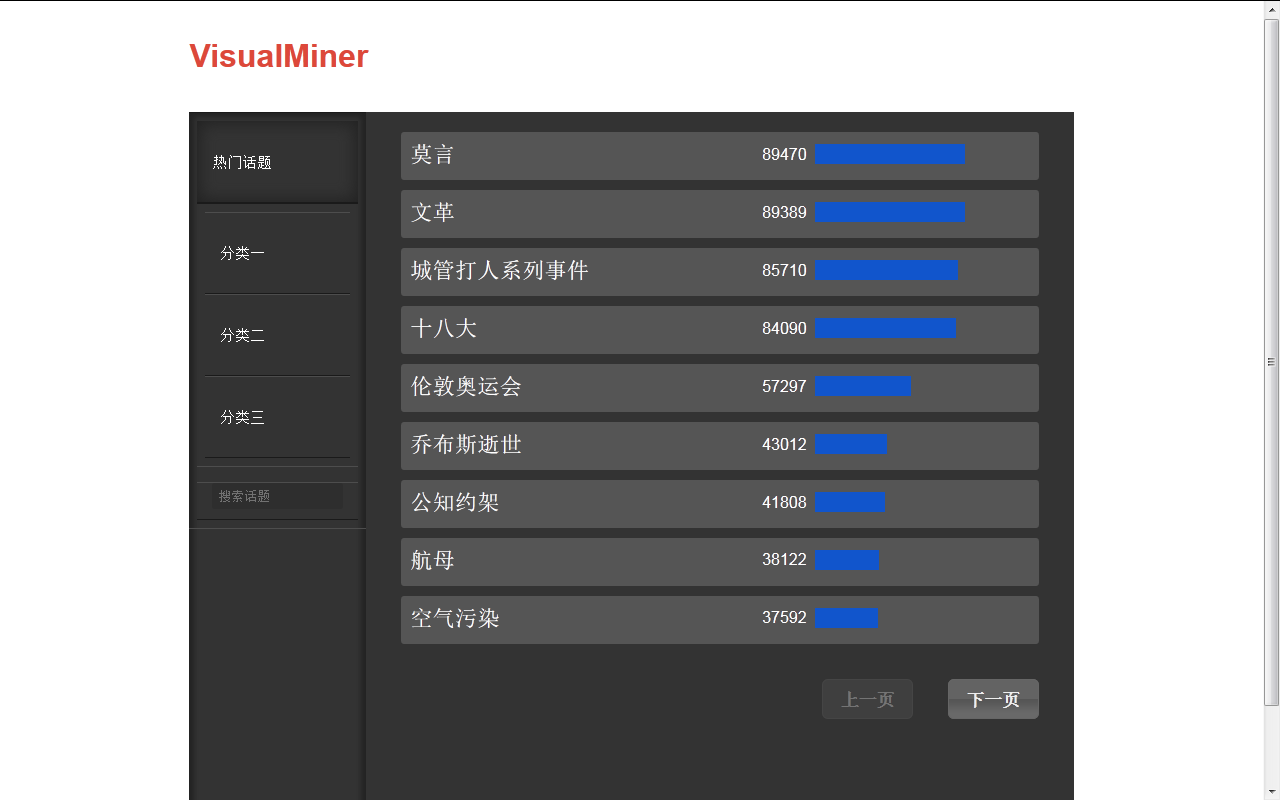
\includegraphics[width=\textwidth, height=0.35\textheight]{show_main}
图 5-1 主页效果
\caption{homepage}
\end{figure}

如图 5-2 是在主页上点击 “玉树地震” 后进入其事件概况页面,包括话题的简介及评论数和转发数和位居前 5 的微博,我们保留了微博的作者和内容。通过这些信息,用户可以清楚地了解一个话题的内容和新浪微博上的主流观点。

\begin {figure}[!h]
\centering
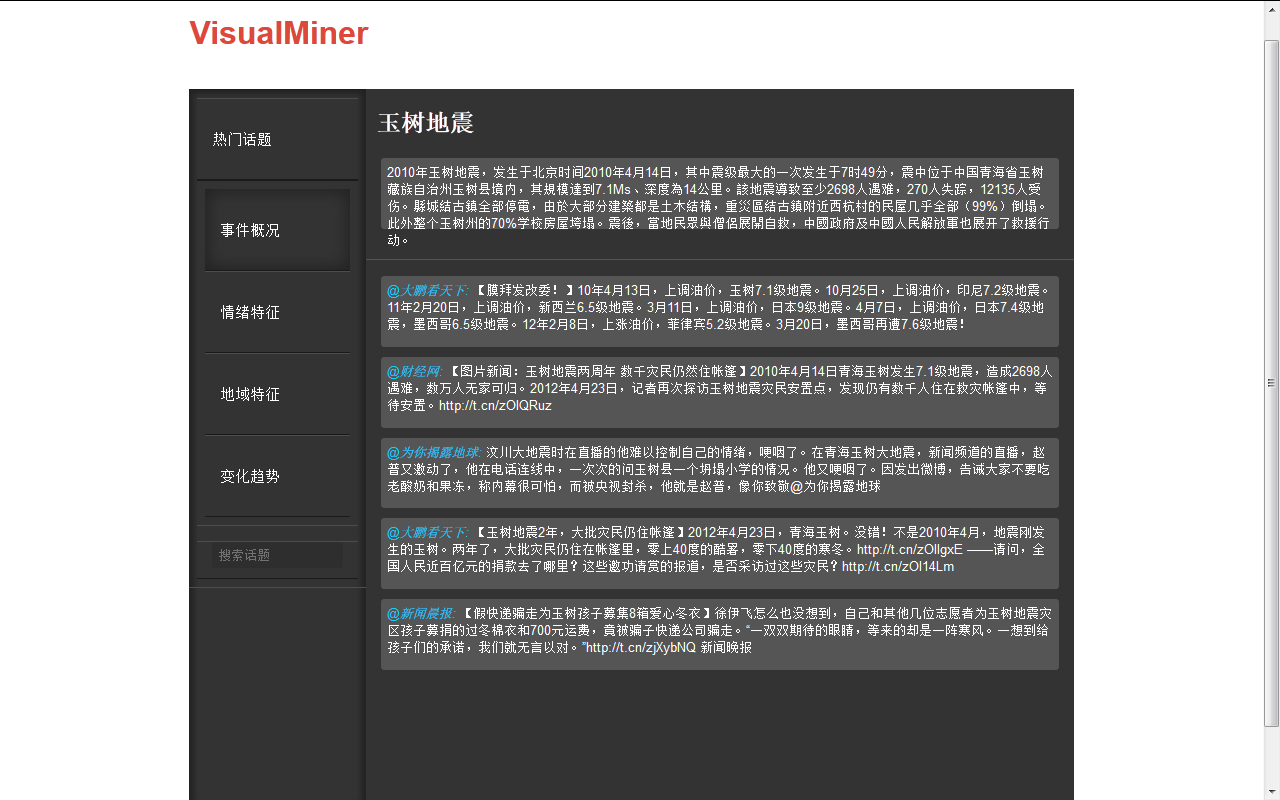
\includegraphics[width=\textwidth, height=0.4\textheight]{show_overview}
图 5-2 事件概况效果
\caption{overview page}
\end{figure}


图 5-3 显示的是新浪微博上关于 “上海11.15大火” 话题的情绪特征页面。通过柱状图,我们可以明显看到 “悲伤” (蓝色)是主导情绪,这和人们一般对灾难的反应相符。排在第二的 “快乐” (快乐)似乎有悖常理,进一步查询右边的情绪词云图可以发现这里 “快乐” 的含义是 “相信”,“美丽”,“共勉” 这些在伤痛中互相勉励,共度难关的词汇。结合情绪特征和情绪词,我们可以推测出人们对这场不幸的主要心态是悲伤中不失信心。

\begin{figure}[!h]
\centering
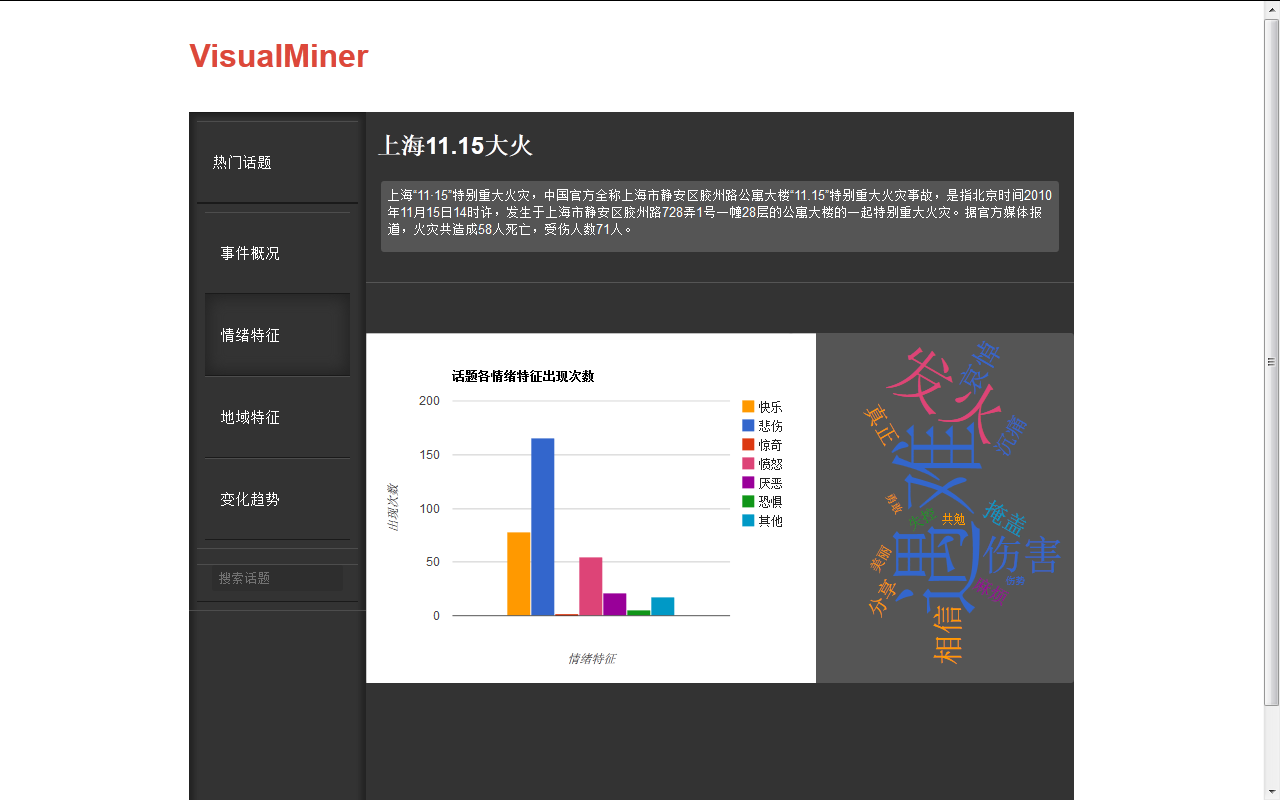
\includegraphics[width=\textwidth, height=0.35\textheight]{show_emotion}
图 5-3 情绪特征效果
\caption{emotion page}
\end{figure}

图 5-4 显示的是新浪微博上关于 “上海11.15大火” 话题的地域分布页面。图上深色区域表示话题讨论数较多的地域。我们可以发现话题的讨论集中在了话题的发生地(“上海”)。注意这仅仅作为参考,不能排除其它地方的微博用户刚好对该话题感兴趣,也不是所有的话题都能呈现出地域差异。
\begin{figure}[!h]
\centering
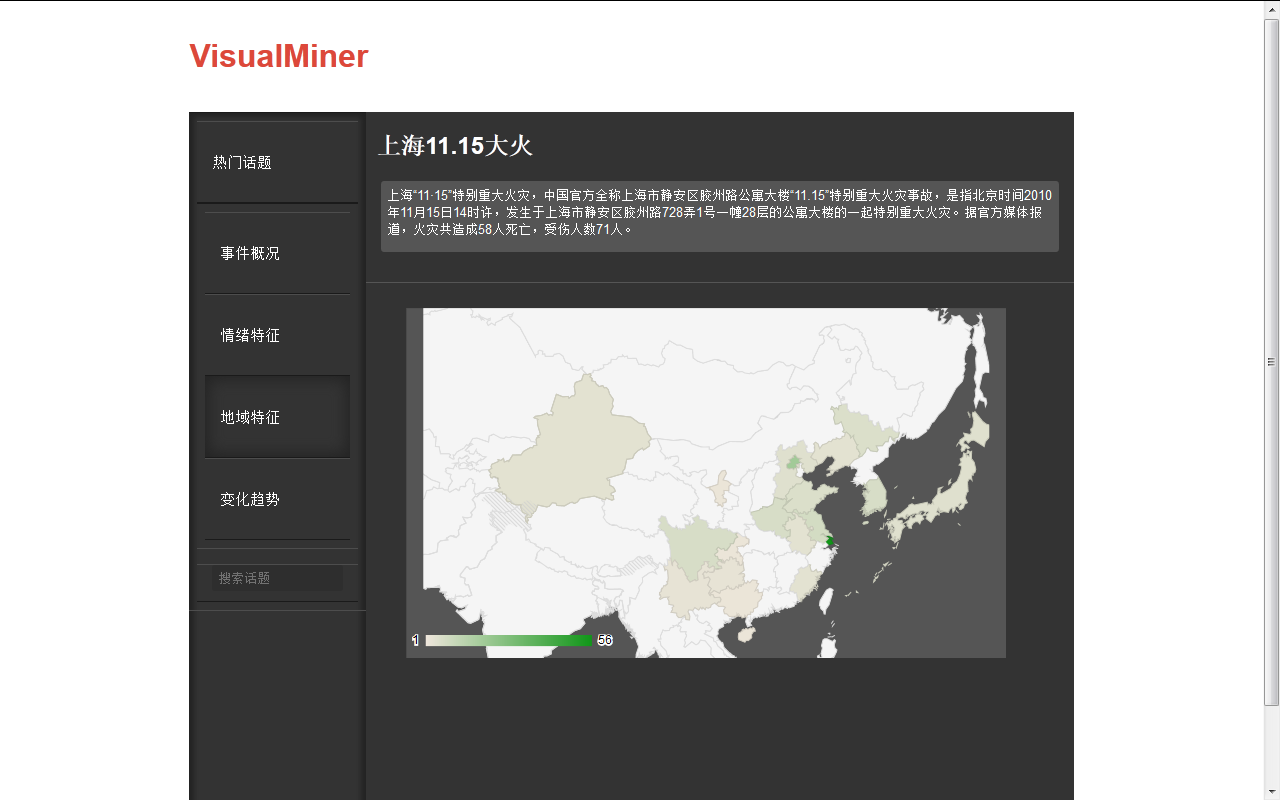
\includegraphics[width=\textwidth, height=0.35\textheight]{show_location}
图 5-4 地域特征效果
\caption{location page}
\end{figure}

图 5-5 显示的是新浪微博上关于 “伦敦奥运会” 话题的变化趋势页面。有关 “伦敦奥运会” 的讨论数在 2012 年 8 月显著上升,随后回落。而那段时间正是伦敦奥运会举办的时间。通过变化趋势图,用户能立即找到话题的起止时间。

\begin{figure}[!h]
\centering
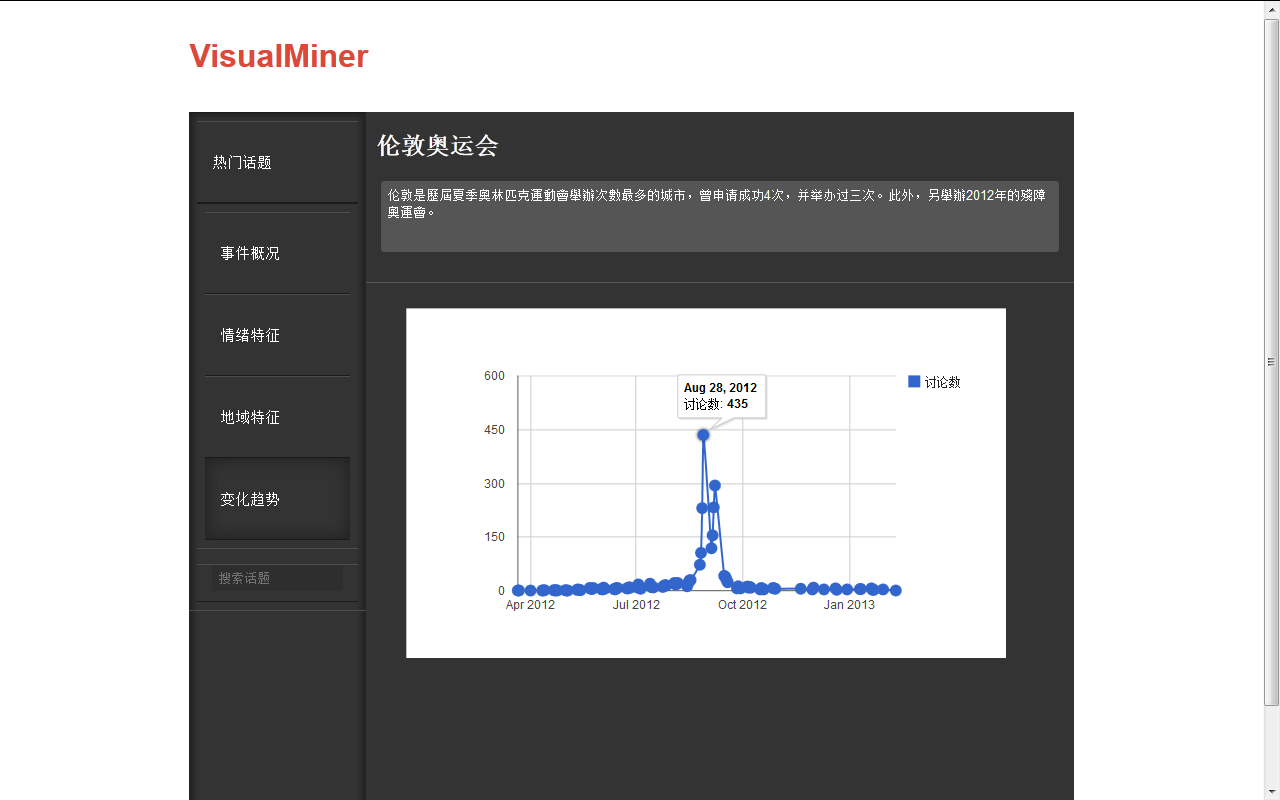
\includegraphics[width=\textwidth, height=0.4\textheight]{show_time}
图 5-5 变化趋势效果
\caption{trend page}
\end{figure}

